%%%%%%%%%%%%%%%%%%%%%%%%%%%%%%%%%%%%%%%%%%%%%%%%%%%%%%%%%%%%%%%%%%%%%%
% Papers Over Time
% Author: Dr.-Ing. Mark Schutera
% Based on Tufte-style layout
%\makeindex % disabled to avoid requiring makeindex/.ind during quick builds
%%%%%%%%%%%%%%%%%%%%%%%%%%%%%%%%%%%%%%%%%%%%%%%%%%%%%%%%%%%%%%%%%%%%%%

\documentclass{../sharedAssets/tufte}

%%
% Book metadata
\title{Papers Over Time}
\author[\defaultauthor]{\defaultauthor}
\publisher[\defaultpublisher]{\defaultpublisher}
\renewcommand{\notesdir}{notes_papersovertime}

% Load optional fonts
\loadoptionalfonts

% Additional packages
\usepackage{pifont}
\usepackage{amsmath}
\usepackage{soul}
\usepackage{textcase}
\usepackage{enumitem}
\usepackage{tikz}
\usetikzlibrary{positioning,arrows.meta}
\usepackage{pgfplots}
\usepackage{float}
\usepackage[maxfloats=256]{morefloats}
\usepackage{algorithm}
\usepackage{algpseudocode}

\extrafloats{100}

\begin{document}

\makestandardfrontmatter
\tableofcontents

\makeintroduction{%
  \newthought{Papers over time} reads the field through its primary literature.
  Each session lifts a single paper, situates it in its moment, and asks what
  it changed and what it left unfinished. The aim is fluency in the genre and
  taste in the questions.
}

\mainmatter
\authorinrectoheader

\chapter{Zebrafish Phenotype Pattern Recognition}\index{zebrafish}\index{phenotype}\index{high-throughput screening}
\printchapterversion{01_zebrafish_phenotype}

\newthought{Counting Embryos}

\marginnote{%
  \begin{flushright}
  \newthought{Automated Phenotype Pattern Recognition of Zebrafish for High-throughput Screening}\\
  Schutera et al.\ (2016)\\
  \textit{Bioengineered} 7(4)\\[4pt]
  {\color{black}\qrcode[height=1.2cm]{https://doi.org/10.1080/21655979.2016.1197710}}
  \end{flushright}%
  \bigskip
  \newthought{Bachelor thesis.}\\
  The first paper, written before any of this was supposed to be a career.%
}

\marginnote{\newthought{Model organism.} Zebrafish (\textit{Danio rerio}) embryos are transparent, cheap, and develop fast. The phenotype is visible at 72 hours post fertilization.}

\newthought{A single screen} produces thousands of embryos. Each one has to be inspected at fixed time points to decide which ones carry the phenotype of interest. By hand, the screen never finishes.

\newthought{Imaging had outpaced scoring.} Embryos could be photographed faster than a biologist could classify them. The bottleneck had moved.

\vspace{3.5em}

\begin{tabular}{p{3.8cm} p{6.5cm}}
    \textbf{Question} &
        Can a classifier replace the human at the microscope? \\[3pt]
    \textbf{Setting} &
        Four phenotypes at 72 hpf, reduced to wild type vs.\ variant. \\[3pt]
    \textbf{Headline} &
        79\% to 99\% accuracy, no user interaction. \\
\end{tabular}

\vspace{3.5em}

\begin{center}
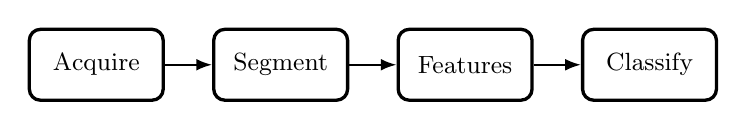
\begin{tikzpicture}[node distance=6mm, every node/.style={font=\small}]
  \tikzset{
    stage/.style={rounded corners, draw, very thick, minimum width=1.7cm, minimum height=0.9cm, align=center},
    arr/.style={-{Latex[length=2mm]}, thick}
  }
  \node[stage] (acq)  {Acquire};
  \node[stage, right=of acq]  (seg)  {Segment};
  \node[stage, right=of seg]  (feat) {Features};
  \node[stage, right=of feat] (cls)  {Classify};
  \draw[arr] (acq)  -- (seg);
  \draw[arr] (seg)  -- (feat);
  \draw[arr] (feat) -- (cls);
\end{tikzpicture}
\end{center}

\vspace{2em}

\marginnote{\newthought{The move.} Treat acquisition and classification as one system. The features the classifier needs are the features the rig is set up to capture.}

\newthought{No deep learning.} The data set is small, the phenotypes are well described by intensity and geometry, and a domain expert can name the features that matter. Classical pattern recognition ships.

\marginnote{\newthought{Take it from here.} Drift across screens, rigs, and batches becomes the dominant problem. Labels become the next bottleneck. The later papers pick the thread up.}

\newthought{The contribution is the loop.} Rig plus software runs unattended on a real screening question and returns numbers a biologist can act on. Algorithm second, system first.


\bibliographystyle{abbrvnat}
\bibliography{papersovertime}

\end{document}
